\section{Вынужденное движение}

Рассмотрим систему 2-го порядка, заданную дифференциальным уравнением
\begin{equation*}
    \ddot y + a_1\dot y + a_0 y = u.
\end{equation*}
Используя немного модицированная схема из лабораторной работы 2 (см. рис. \ref{fig:task_1_slx}),
были проведены 27 симуляций для трех наборов коэффициентов $a_1$ и $a_0$:
\begin{itemize}
    \item $a_1 = 2.4, a_0 = 101.44$;
    \item $a_1 = 0, a_0 = 100$;
    \item $a_1 = -2.4, a_0 = 101.44$;
\end{itemize}
трех случаев начальных условий:
\begin{itemize}
    \item $y(0) = -1$, $\dot y(0) = 0$;
    \item $y(0) = 0$, $\dot y(0) = 0$;
    \item $y(0) = 1$, $\dot y(0) = 0$;
\end{itemize}
и трех входных воздействий:
\begin{itemize}
    \item $u(t) = 2.5$;
    \item $u(t) = 0.8t$;
    \item $u(t) = \sin 8t$;
\end{itemize}
графики которых можно увидеть на рисунках \ref{fig:task_1_out_1}, \ref{fig:task_1_out_2}, \ref{fig:task_1_out_3},
а также на рисунках \ref{fig:task_1_out_11} и \ref{fig:task_1_out_21}, в которых увеличено время симуляции,
на отдельном ресунке один набор коэффициентов и три входных воздействия, на каждом графике отображены
три набора начальных условий. Смотря на эти графики можно увидеть, что константный вход
не изменяет тип устойчивости систем, линейное сделало все системы неустойчивыми, а
грамоническое сделало из асимптотически устойчивых устойчивые по Ляпунову.

\begin{figure}
    \centering
    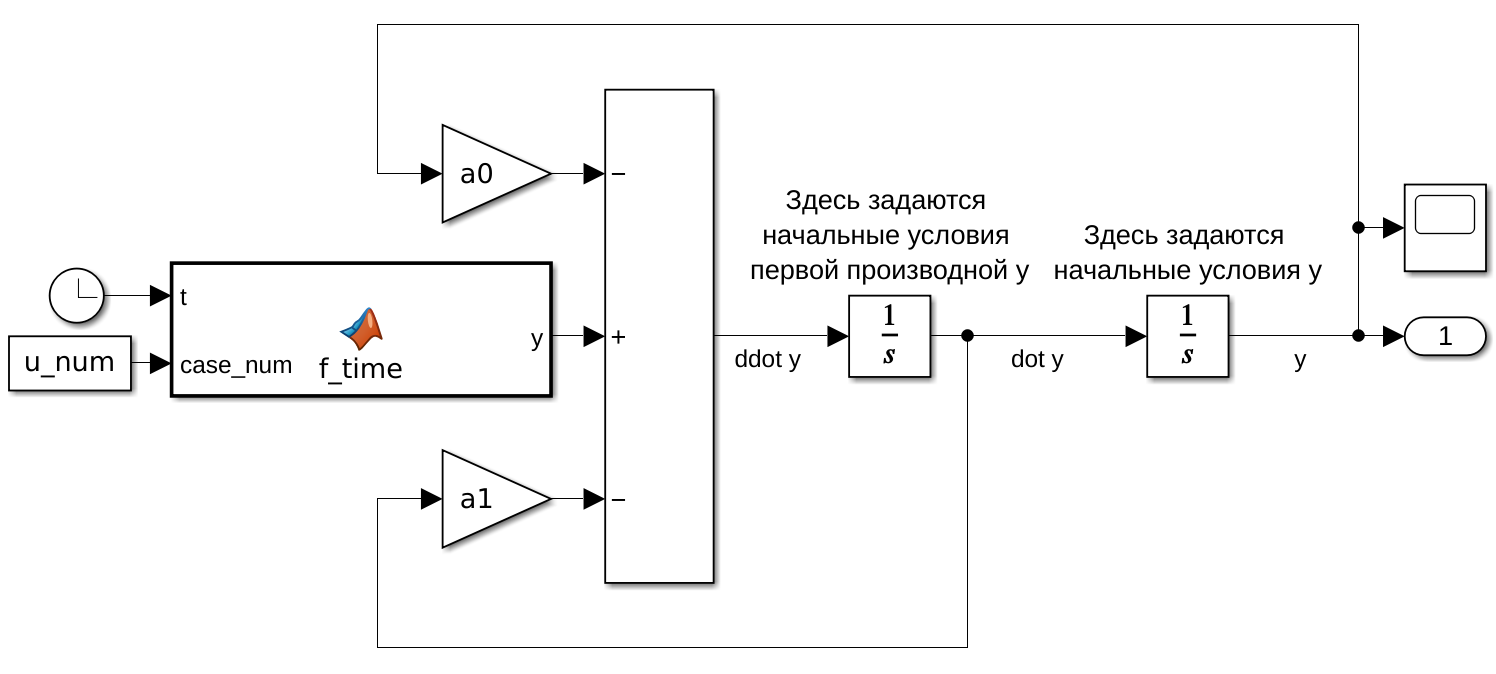
\includegraphics[width=0.9\textwidth]{figs/task_1_slx.png}
    \caption{Структурная схема дифференциального уравнения задания 1.}
    \label{fig:task_1_slx}
\end{figure}

\begin{figure}
    \centering
    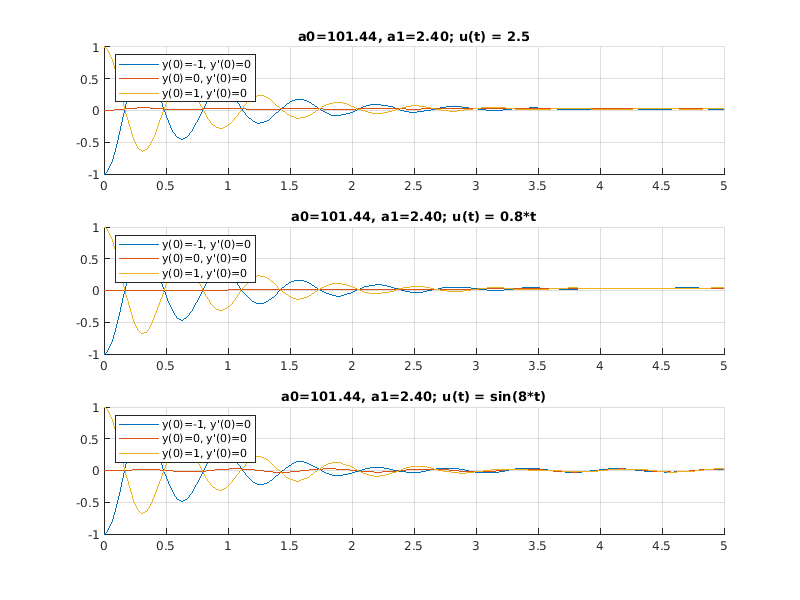
\includegraphics[width=0.9\textwidth]{figs/task_1_out_1.png}
    \caption{Результаты симуляции для $a_1 = 2.4, a_0 = 101.44$ и $u(t) = 2.5$.}
    \label{fig:task_1_out_1}
\end{figure}

\begin{figure}
    \centering
    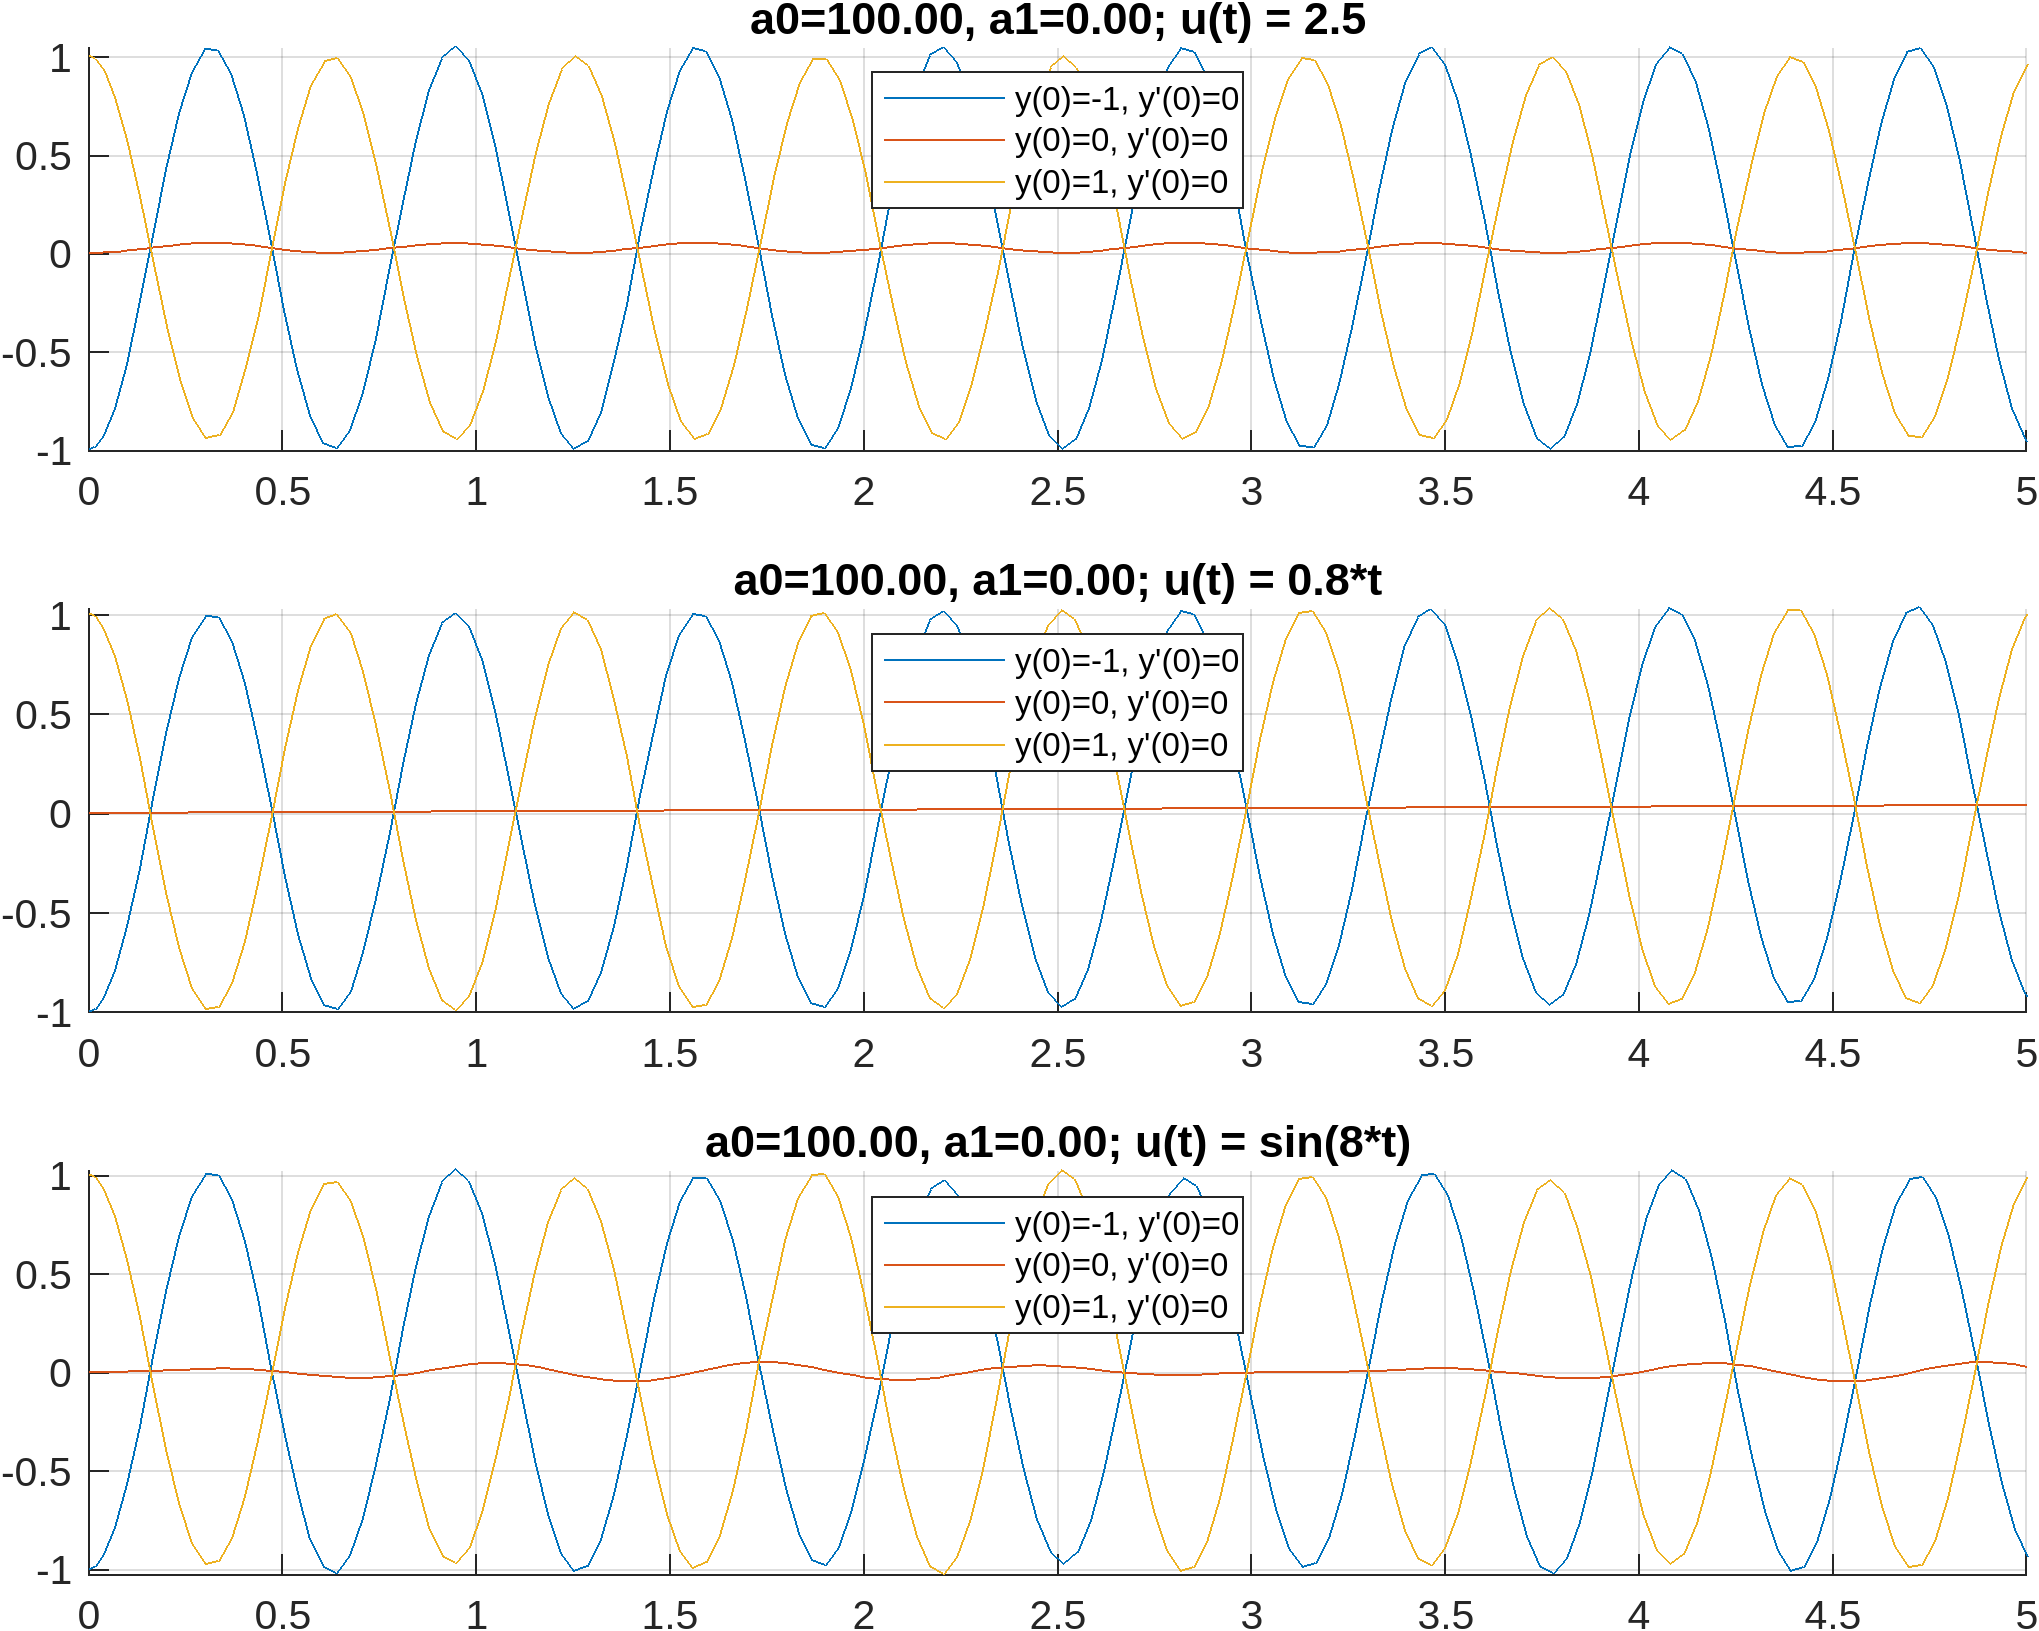
\includegraphics[width=0.9\textwidth]{figs/task_1_out_2.png}
    \caption{Результаты симуляции для $a_1 = 0, a_0 = 100$ и $u(t) = 0.8t$.}
    \label{fig:task_1_out_2}
\end{figure}

\begin{figure}
    \centering
    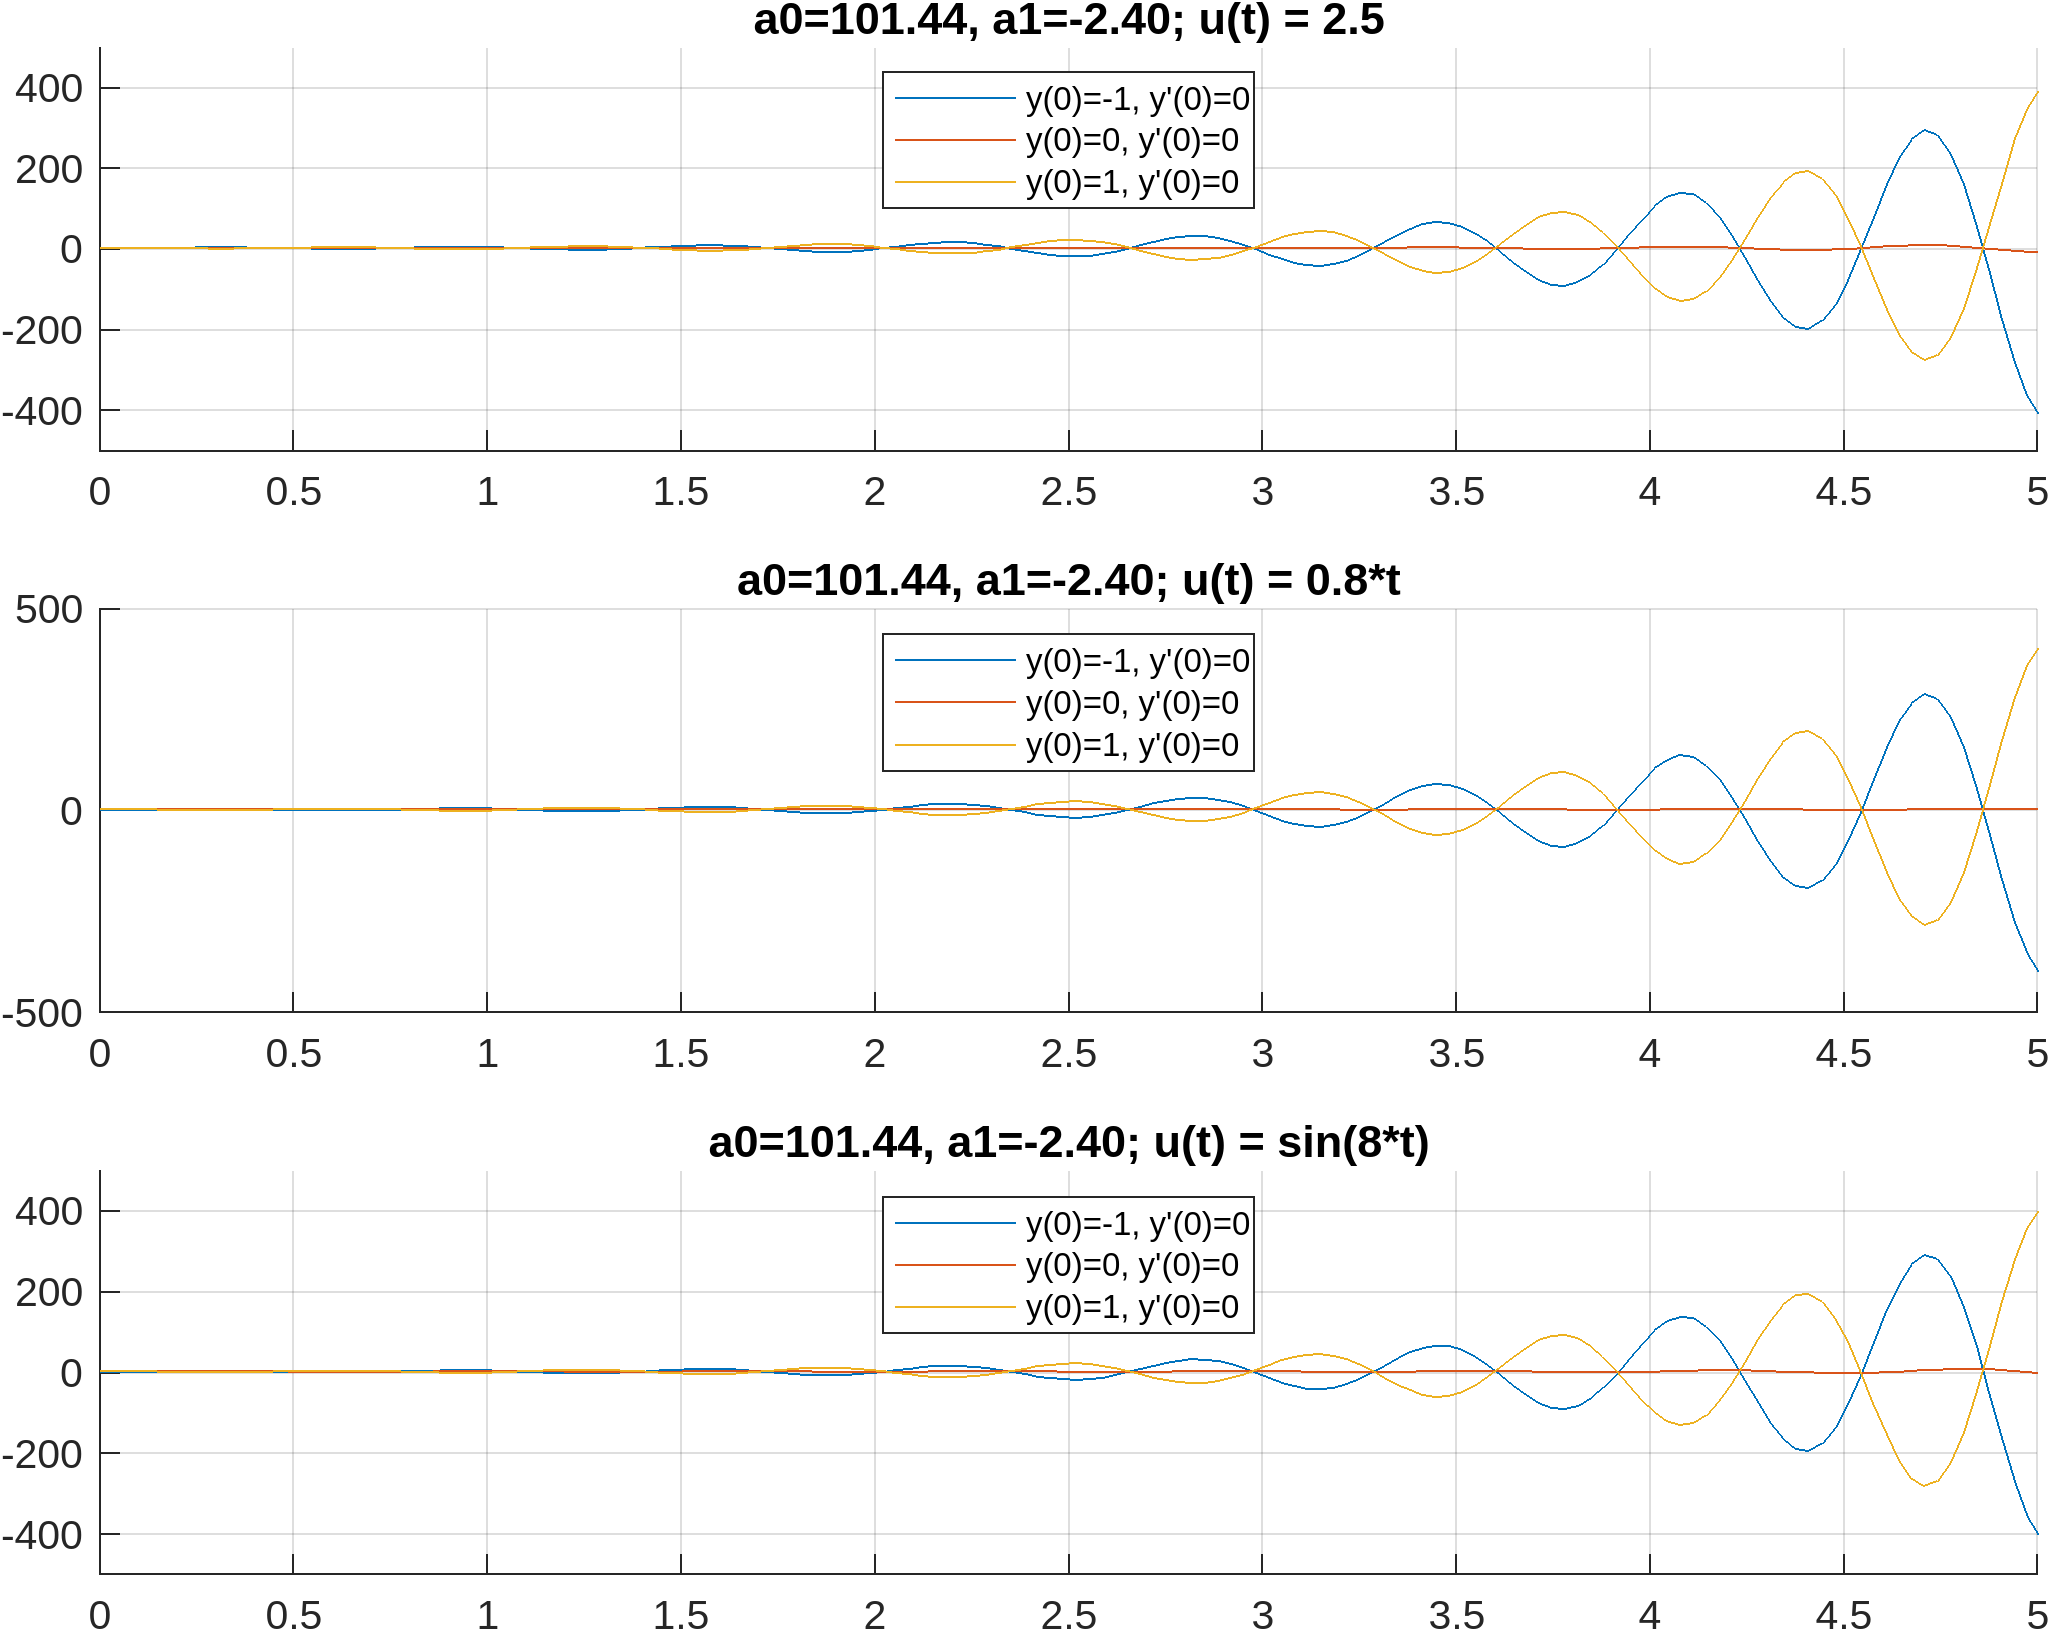
\includegraphics[width=0.9\textwidth]{figs/task_1_out_3.png}
    \caption{Результаты симуляции для $a_1 = -2.4, a_0 = 101.44$ и $u(t) = \sin 8t$.}
    \label{fig:task_1_out_3}
\end{figure}

\begin{figure}
    \centering
    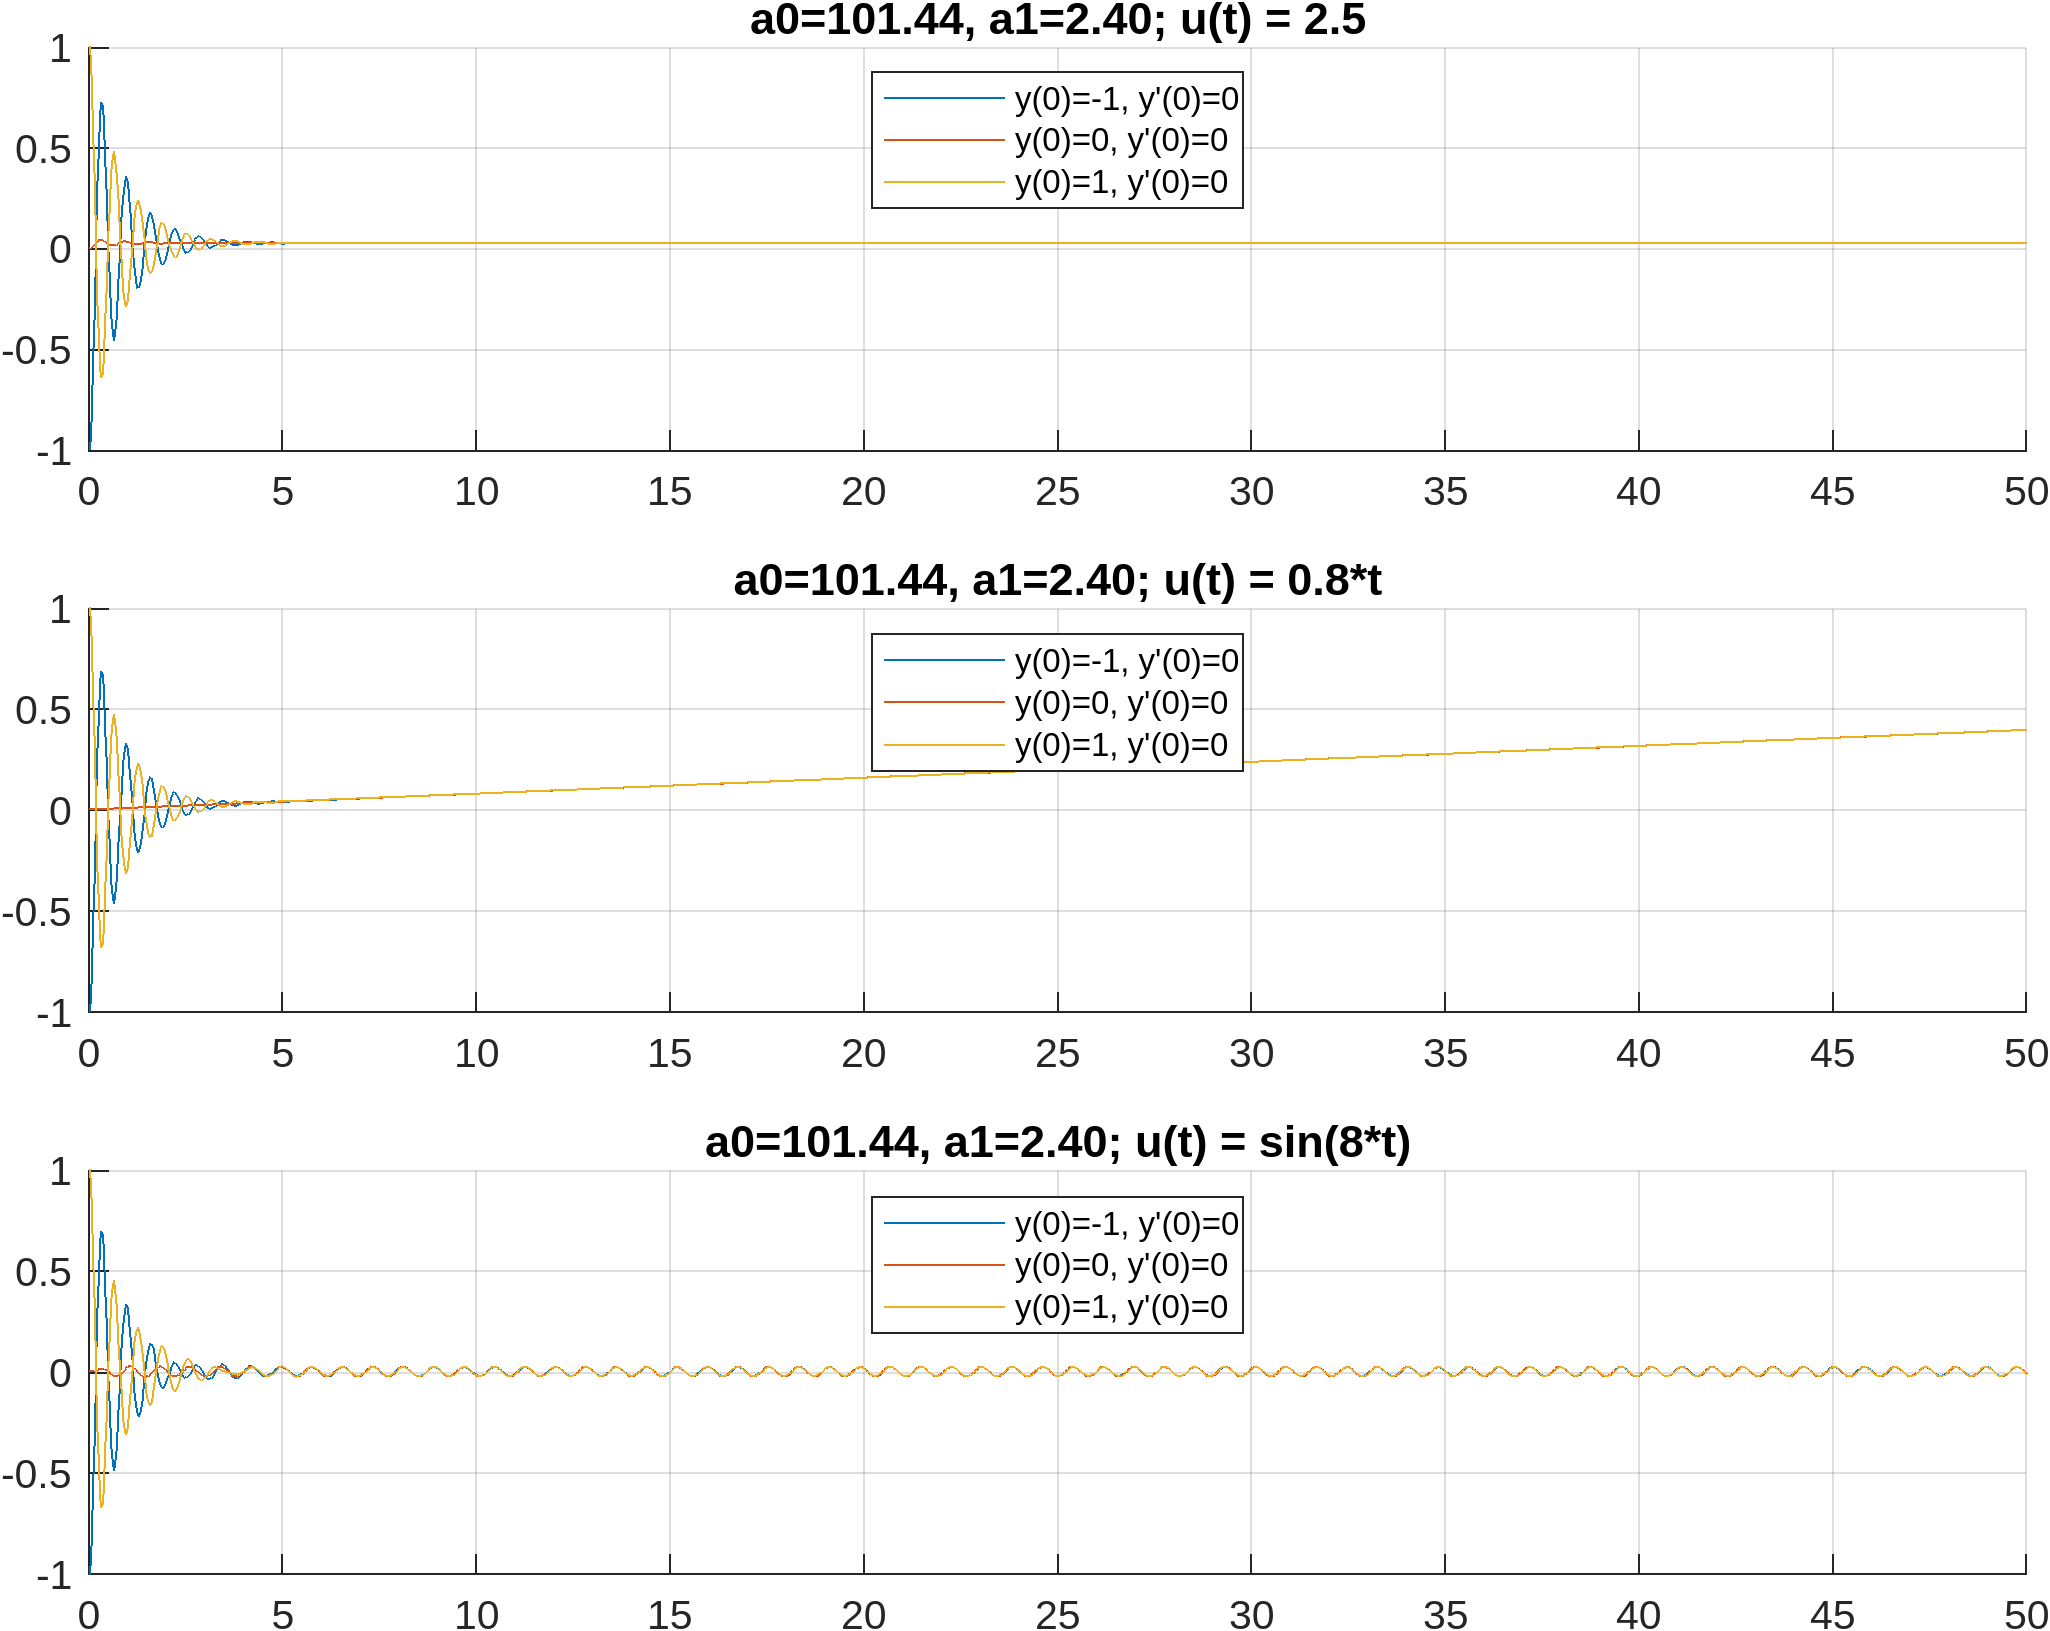
\includegraphics[width=0.9\textwidth]{figs/task_1_out_11.png}
    \caption{Результаты симуляции 50 секунд для $a_1 = 2.4, a_0 = 101.44$ и $u(t) = 2.5$.}
    \label{fig:task_1_out_11}
\end{figure}

\begin{figure}
    \centering
    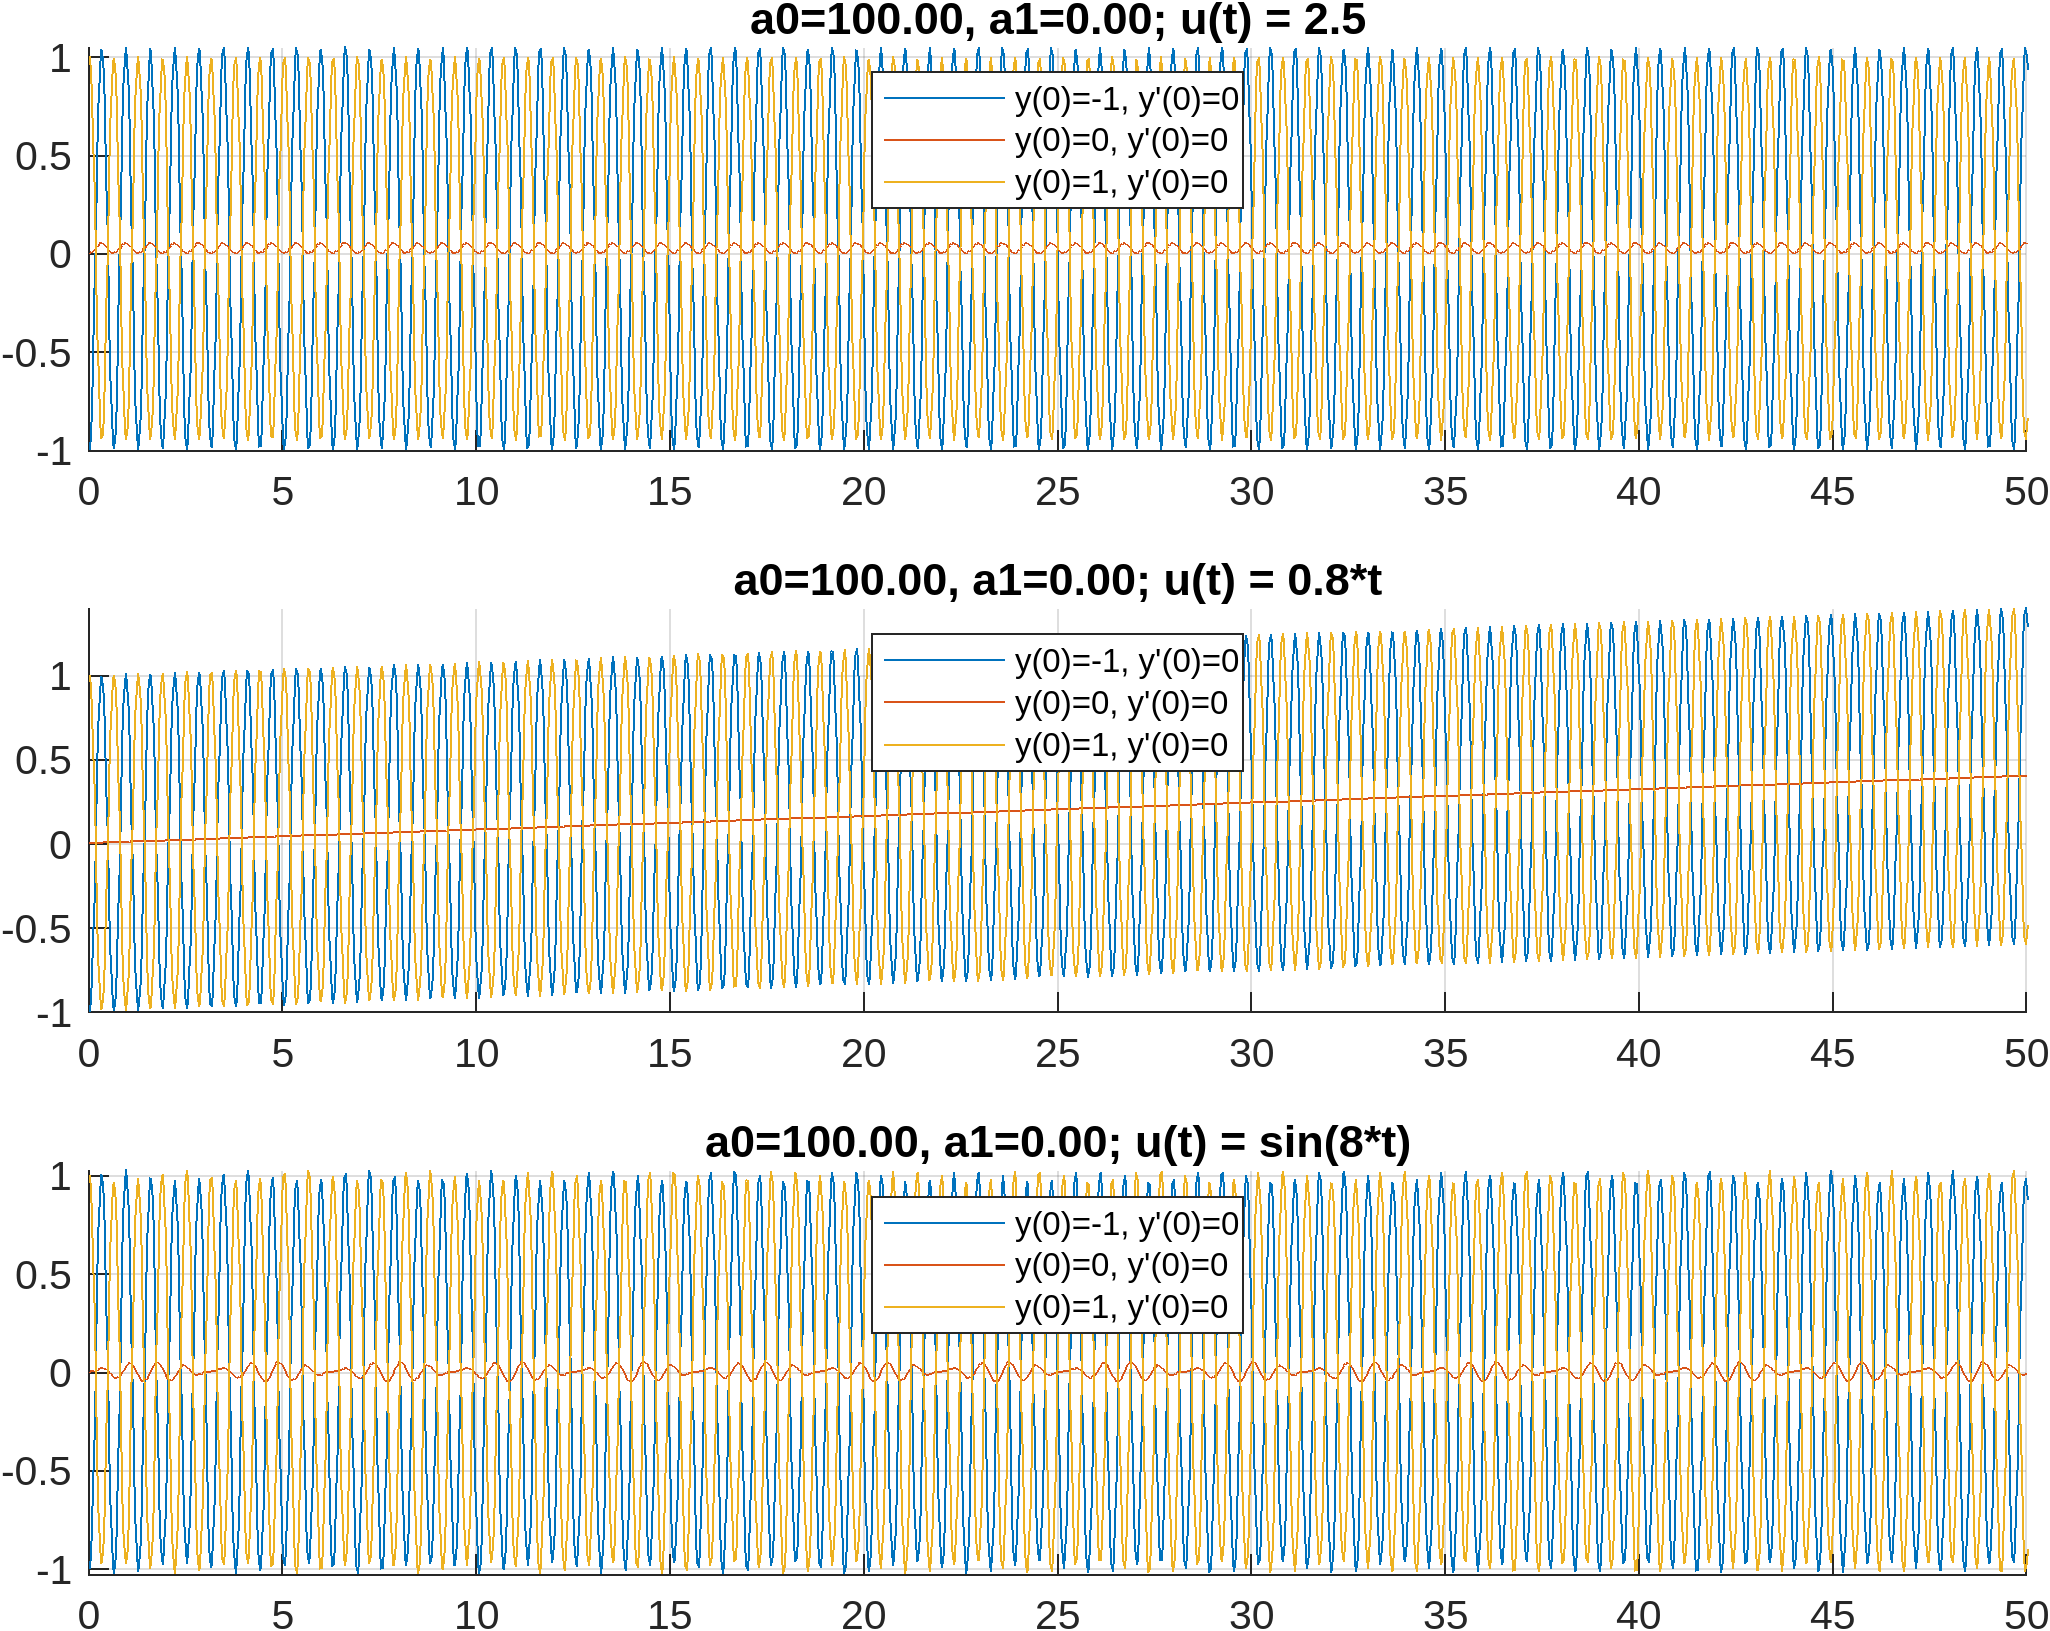
\includegraphics[width=0.9\textwidth]{figs/task_1_out_21.png}
    \caption{Результаты симуляции 50 секунд для $a_1 = 0, a_0 = 100$ и $u(t) = 0.8t$.}
    \label{fig:task_1_out_21}
\end{figure}


\newpage
\section{Качество переходных процессов}

Имеем систему 3-го порядка, заданной передаточной функцией
\begin{equation*}
    W(s)=\frac{|\lambda_1 \lambda_2 \lambda_3|}{(s-\lambda_1)(s-\lambda_2)(s-\lambda_3)},
\end{equation*}
исследуем зависимость качества переходной характеристики от выбора полюсов передаточной 
функции. Для этого зададимся 10 наборами полюсов $\lambda_1, \lambda_2, \lambda_3$ с
отрицательной вещественной частью, их можно увидеть в таблице \ref{table:task_2}.
Использовалась функция \textit{step} в \textit{MATLAB} для моделирования переходного процесса,
в результате которого получили показатели оценки качества, такие как время переходного процесса
и перерегулирование, значение которых для каждого набора полюсов можно увидеть в таблице \ref{table:task_2},
а графики процессов, на которых черной пунктирной линией отмечена двухпроцентная зона для определения
время переходного процесса, красной - само время передного процесса, и полюсов на комплексной плоскости можно посмотреть на рисунках
с \ref{fig:task_2_out_1} по \ref{fig:task_2_out_10}. 

Сначало были выбраны чисто реальные небольшие полюса (см. рисунок \ref{fig:task_2_out_1}), и процесс завершается за 7.5 секунд без какого либо
перерегулирования, затем на графиках с \ref{fig:task_2_out_2} по \ref{fig:task_2_out_5} увеличивалась
реальная часть лямбд, и можно увидеть, что время переходного процесса уменьшалось влоть до 0.15
секунд, где $\lambda_1 = -50$, $\lambda_2 = -50$, $\lambda_3 = -50$, перерегулирование осталось нулевым.
Далее добавлялась мнимая часть при сохранении небольшой вещественной части, на рисунках
с \ref{fig:task_2_out_6} и \ref{fig:task_2_out_7} можно увидеть, что появились колебания, и
чем больше комплексная часть, тем больше частота колебаний, передегулирование осталось нулевым,
время переходного процесса (4 с. и 3.9 с.) по сравнению с первым набором, где такие же вещественные части у полюсов,
уменьшилось почти в два раза (7.5 секунд и 4 секунд). Следующим увеличим вещественную часть (было -1 стало -30),
оставив остальное как в предыдущих двух случах, на рисунках с \ref{fig:task_2_out_8} и \ref{fig:task_2_out_9}
появилось сильное перерегулирование (68\% и 42\%), время переходного процесса уменьшилось
(3.8 с. и 3.2 с.). И последний рисунок \ref{fig:task_2_out_10}, его параметры как на рисунке 
\ref{fig:task_2_out_5}, только комплексная часть теперь 50 вместо 0, и время перехода
уменьшилось в 47 раз, перегулирования нет. 

Подытожим: \textbf{меньшие реальные полюса} обеспечивают медленный и плавный переходной процесс без перерегулирования.
\textbf{Увеличение реальной части} значительно сокращает время переходного процесса, не вызывая перерегулирования.
\textbf{Добавление мнимой части} вводит колебания, сокращает время перехода, но при небольших значениях 
вещественной части перерегулирование отсутствует.
\textbf{Большие реальные и мнимые части одновременно} уменьшают время перехода и для появления
перерегулирования или хотя бы каких-то колебаний нужна еще большая мнимая часть, из чего делаю
вывод, что для появления колебаний нужно определенное соотношение мнимой и вещественной частей.


\begin{table}[ht]
    \centering
    \begin{tabular}{|c|c|c|c|c|}
    \hline
    $\lambda_1$ & $\lambda_2$ & $\lambda_3$ & Время переходного процесса & Перерегулирование \\ \hline
    -1 & -1 & -1 & 7.5166 & 0 \\ \hline
    -10 & -1 & -1 & 5.9383 & 0 \\ \hline
    -30 & -1 & -1 & 5.8677 & 0 \\ \hline
    -50 & -50 & -1 & 3.9524 & 0 \\ \hline
    -50 & -50 & -50 & 0.1504 & 0 \\ \hline
    $-1 + 10i$ & $-1 - 10i$ & -1 & 3.9990 & 0 \\ \hline
    $-1 + 50i$ & $-1 - 50i$ & -1 & 3.9247 & 0 \\ \hline
    $-1 + 10i$ & $-1 - 10i$ & -30 & 3.8445 & 0.6834 \\ \hline
    $-1 + 50i$ & $-1 - 50i$ & -30 & 3.2302 & 0.4227 \\ \hline
    $-50 + 50i$ & $-50 - 50i$ & -50 & 0.0861 & 0 \\ \hline
    \end{tabular}
    \caption{\label{table:task_2}Результаты моделирования для различных наборов полюсов}
\end{table}

\begin{figure}
    \centering
    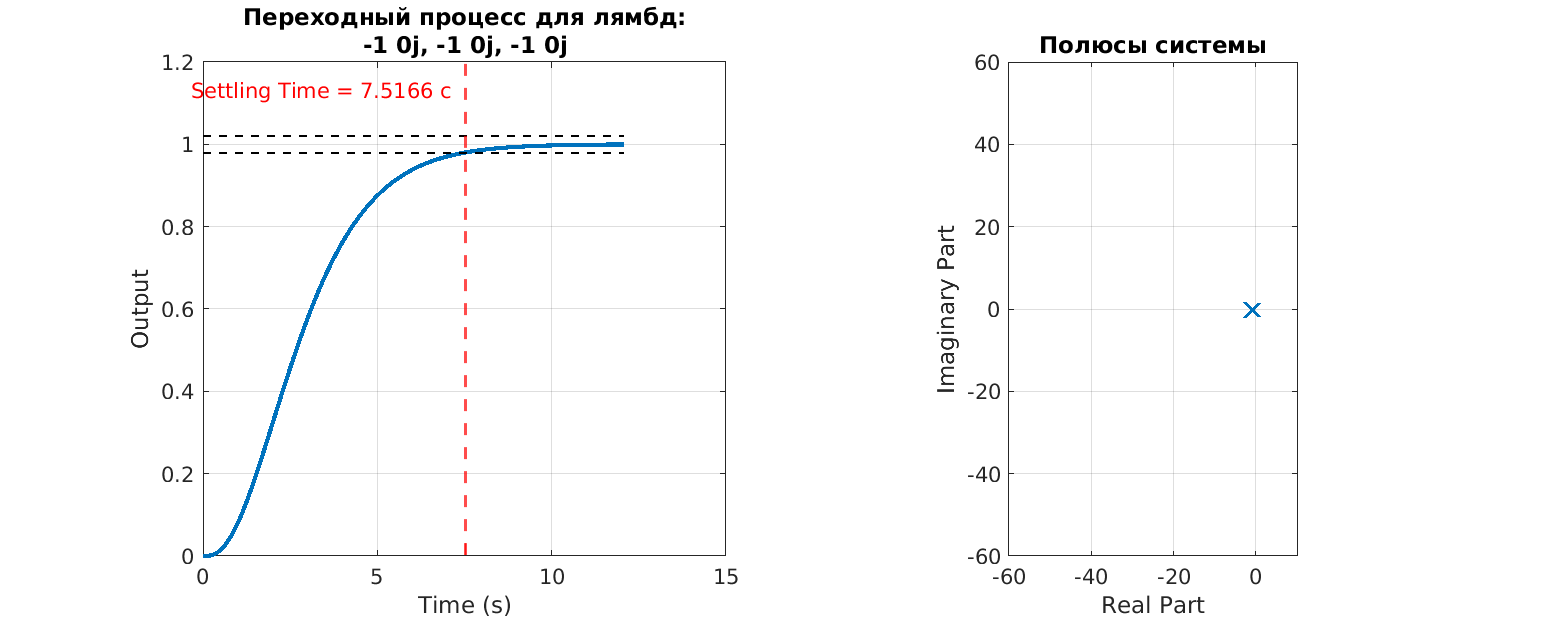
\includegraphics[width=1\textwidth]{figs/task_2_out_1.png}
    \caption{Переходная функция для набора полюсов $\lambda_1 = -1, \lambda_2 = -1, \lambda_3 = -1$.}
    \label{fig:task_2_out_1}
\end{figure}

\begin{figure}
    \centering
    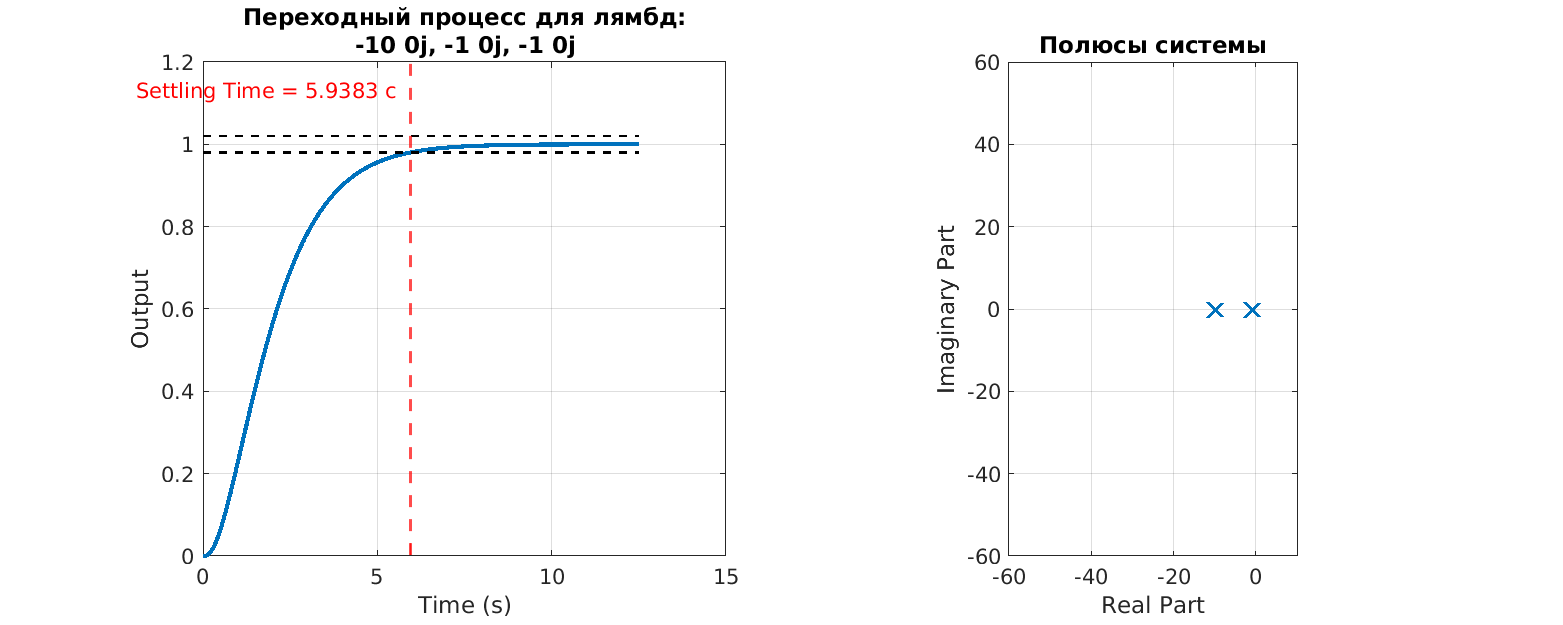
\includegraphics[width=1\textwidth]{figs/task_2_out_2.png}
    \caption{Переходная функция для набора полюсов $\lambda_1 = -10, \lambda_2 = -1, \lambda_3 = -1$.}
    \label{fig:task_2_out_2}
\end{figure}

\begin{figure}
    \centering
    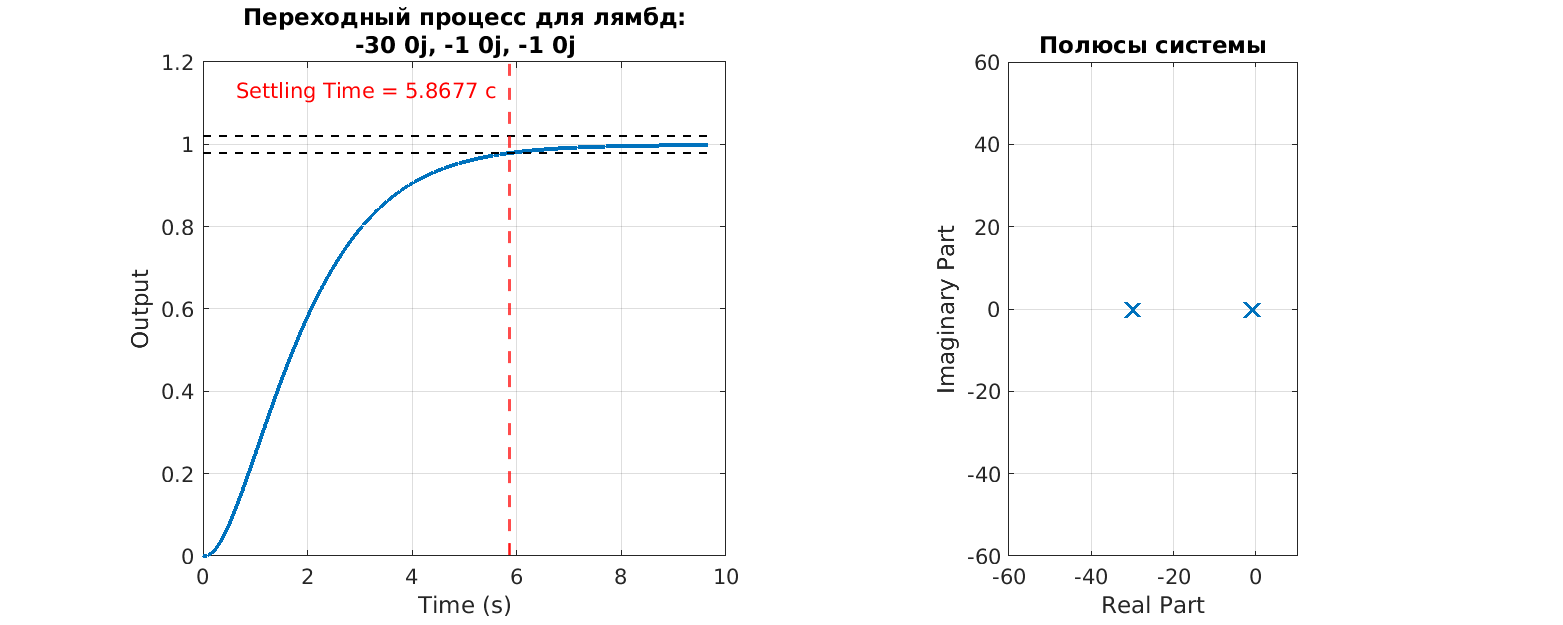
\includegraphics[width=1\textwidth]{figs/task_2_out_3.png}
    \caption{Переходная функция для набора полюсов $\lambda_1 = -30, \lambda_2 = -1, \lambda_3 = -1$.}
    \label{fig:task_2_out_3}
\end{figure}

\begin{figure}
    \centering
    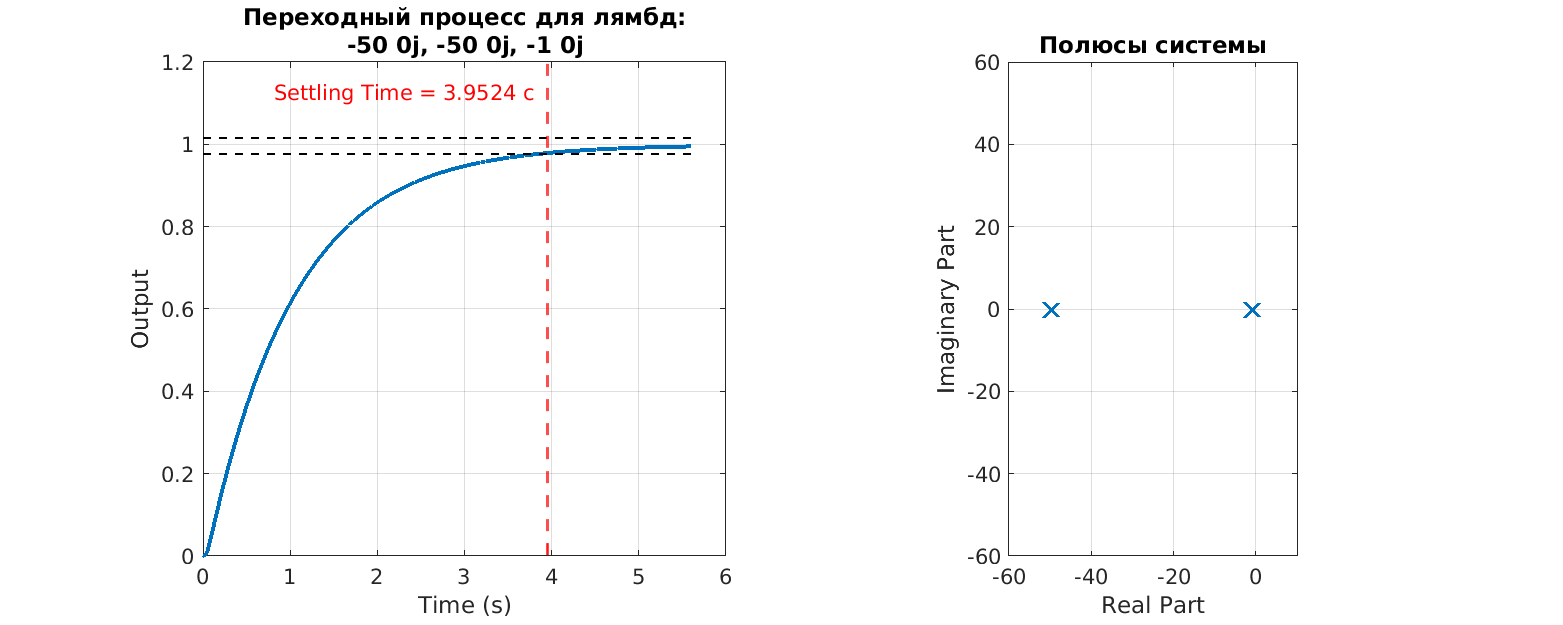
\includegraphics[width=1\textwidth]{figs/task_2_out_4.png}
    \caption{Переходная функция для набора полюсов $\lambda_1 = -30, \lambda_2 = -1, \lambda_3 = -1$.}
    \label{fig:task_2_out_4}
\end{figure}

\begin{figure}
    \centering
    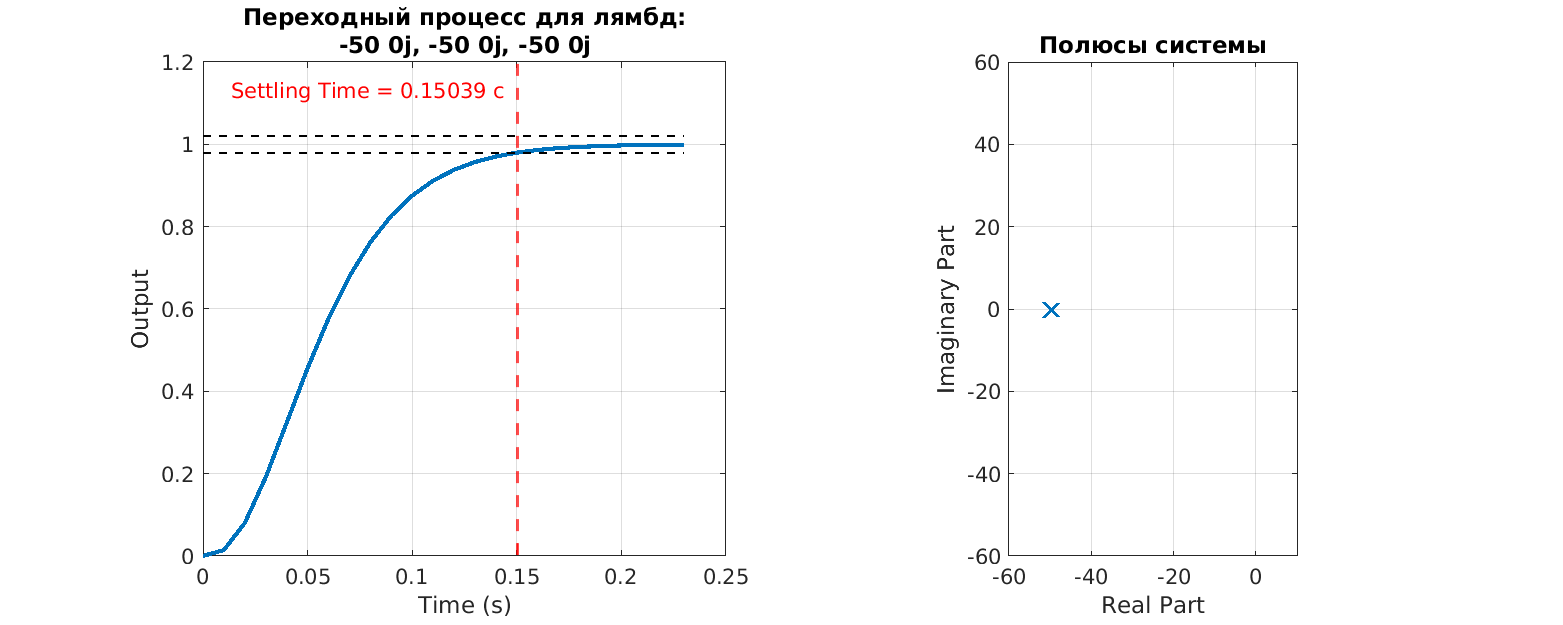
\includegraphics[width=1\textwidth]{figs/task_2_out_5.png}
    \caption{Переходная функция для набора полюсов $\lambda_1 = -5, \lambda_2 = -50, \lambda_3 = -50$.}
    \label{fig:task_2_out_5}
\end{figure}

\begin{figure}
    \centering
    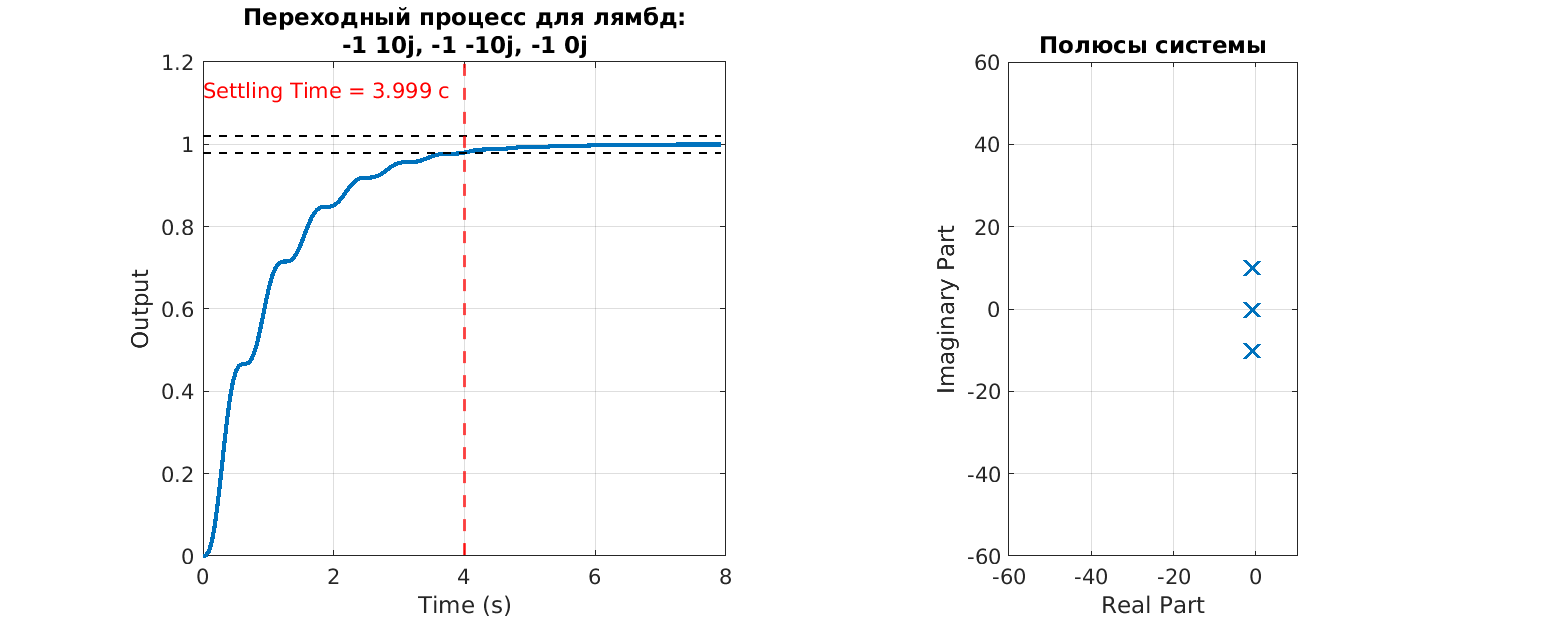
\includegraphics[width=1\textwidth]{figs/task_2_out_6.png}
    \caption{Переходная функция для набора полюсов $\lambda_1 = -1+10i, \lambda_2 = -1 - 10i, \lambda_3 = -1$.}
    \label{fig:task_2_out_6}
\end{figure}

\begin{figure}
    \centering
    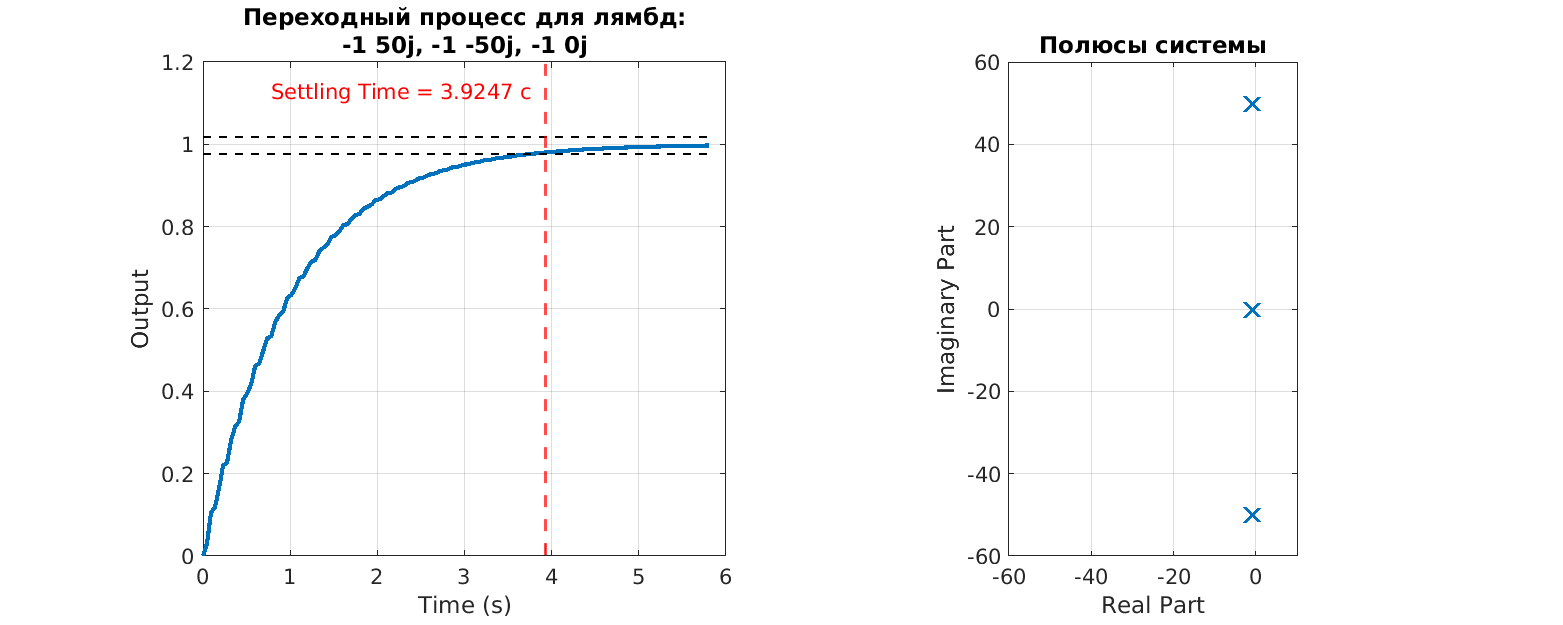
\includegraphics[width=1\textwidth]{figs/task_2_out_7.png}
    \caption{Переходная функция для набора полюсов $\lambda_1 = -1+50i, \lambda_2 = -1 - 50i, \lambda_3 = -1$.}
    \label{fig:task_2_out_7}
\end{figure}

\begin{figure}
    \centering
    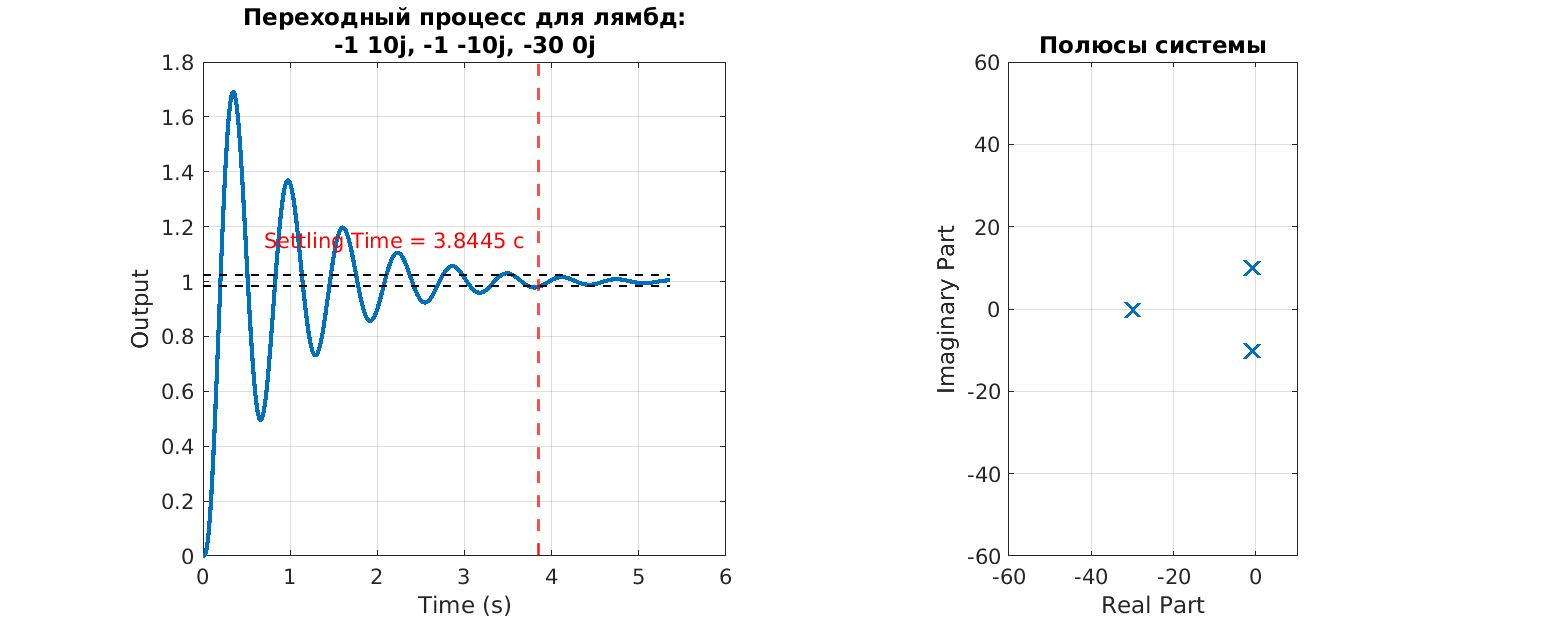
\includegraphics[width=1\textwidth]{figs/task_2_out_8.png}
    \caption{Переходная функция для набора полюсов $\lambda_1 = -1+10i, \lambda_2 = -1 - 10i, \lambda_3 = -30$.}
    \label{fig:task_2_out_8}
\end{figure}

\begin{figure}
    \centering
    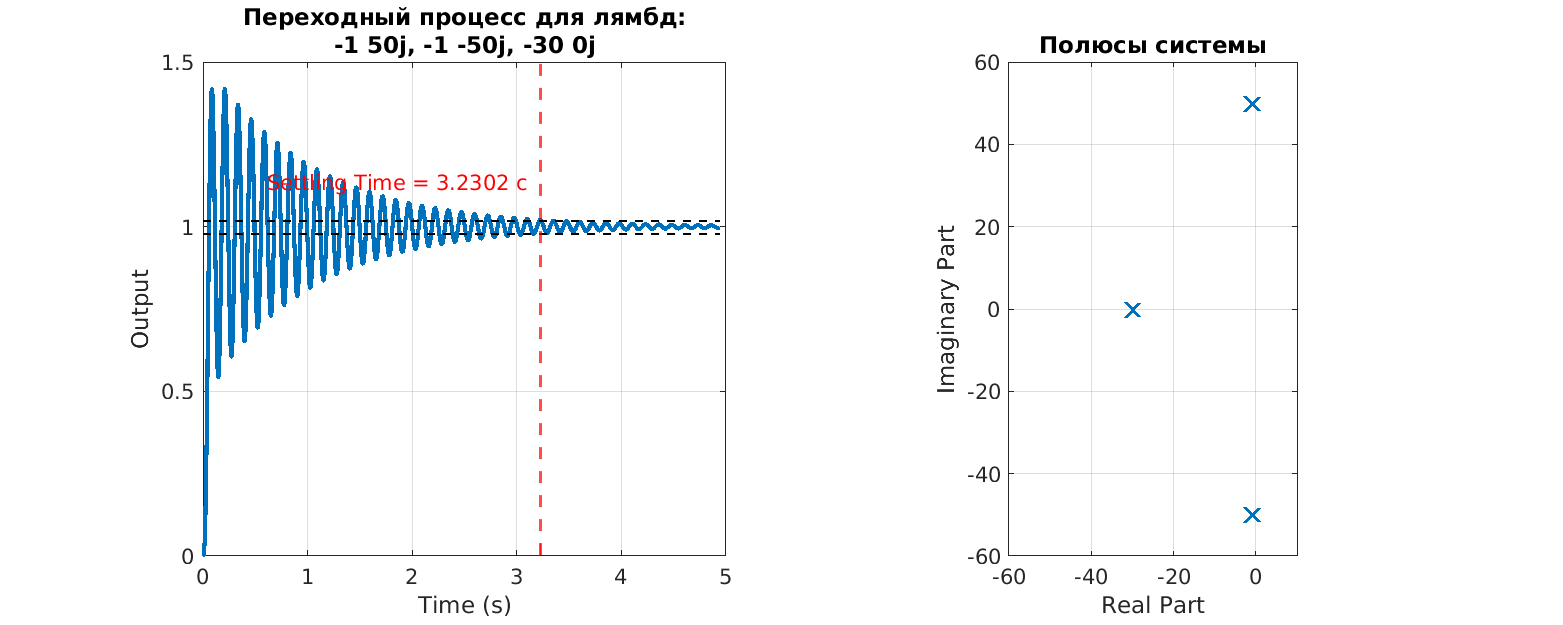
\includegraphics[width=1\textwidth]{figs/task_2_out_9.png}
    \caption{Переходная функция для набора полюсов $\lambda_1 = -1+50i, \lambda_2 = -1 - 50i, \lambda_3 = -30$.}
    \label{fig:task_2_out_9}
\end{figure}

\begin{figure}
    \centering
    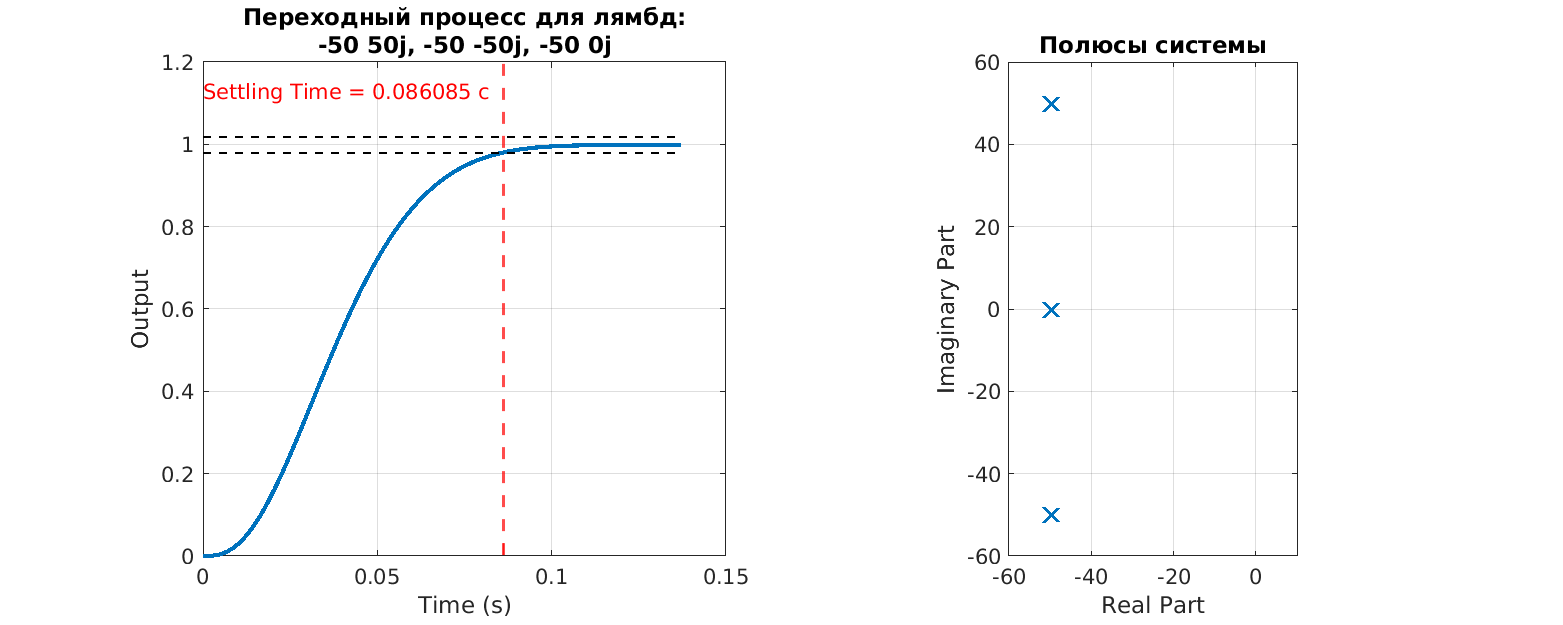
\includegraphics[width=1\textwidth]{figs/task_2_out_10.png}
    \caption{Переходная функция для набора полюсов $\lambda_1 = -50+50i, \lambda_2 = -50 - 50i, \lambda_3 = -50$.}
    \label{fig:task_2_out_10}
\end{figure}



\section*{Вывод}

В лабораторной работе было рассмотрено дифференциальное уравнение второго порядка с
различными коэффициентами, начальными условиями и входными воздействиями, исследовано
влияние вынужденного возмущения на тип сходимости; было исследовано влияние различных
полюсов на переходную характеристику.